\section{Genomförande}
Modellprovaren skrevs i prolog då det är ett lämpligt programmeringsspråk för bevissökning. De befintliga reglerna för CTL implementerades. Vissa av reglerna kräver variabelt antal premisser och detta måste hanteras av programmet. Implementationen av reglerna och modellprovaren gås igenom i kapitel~\ref{sub:modellprovaren}. I kapitel~\ref{sub:modell} beskrivs vår egenvalda modell som föreställer ett trafikljus.

\begin{figure}[hb]
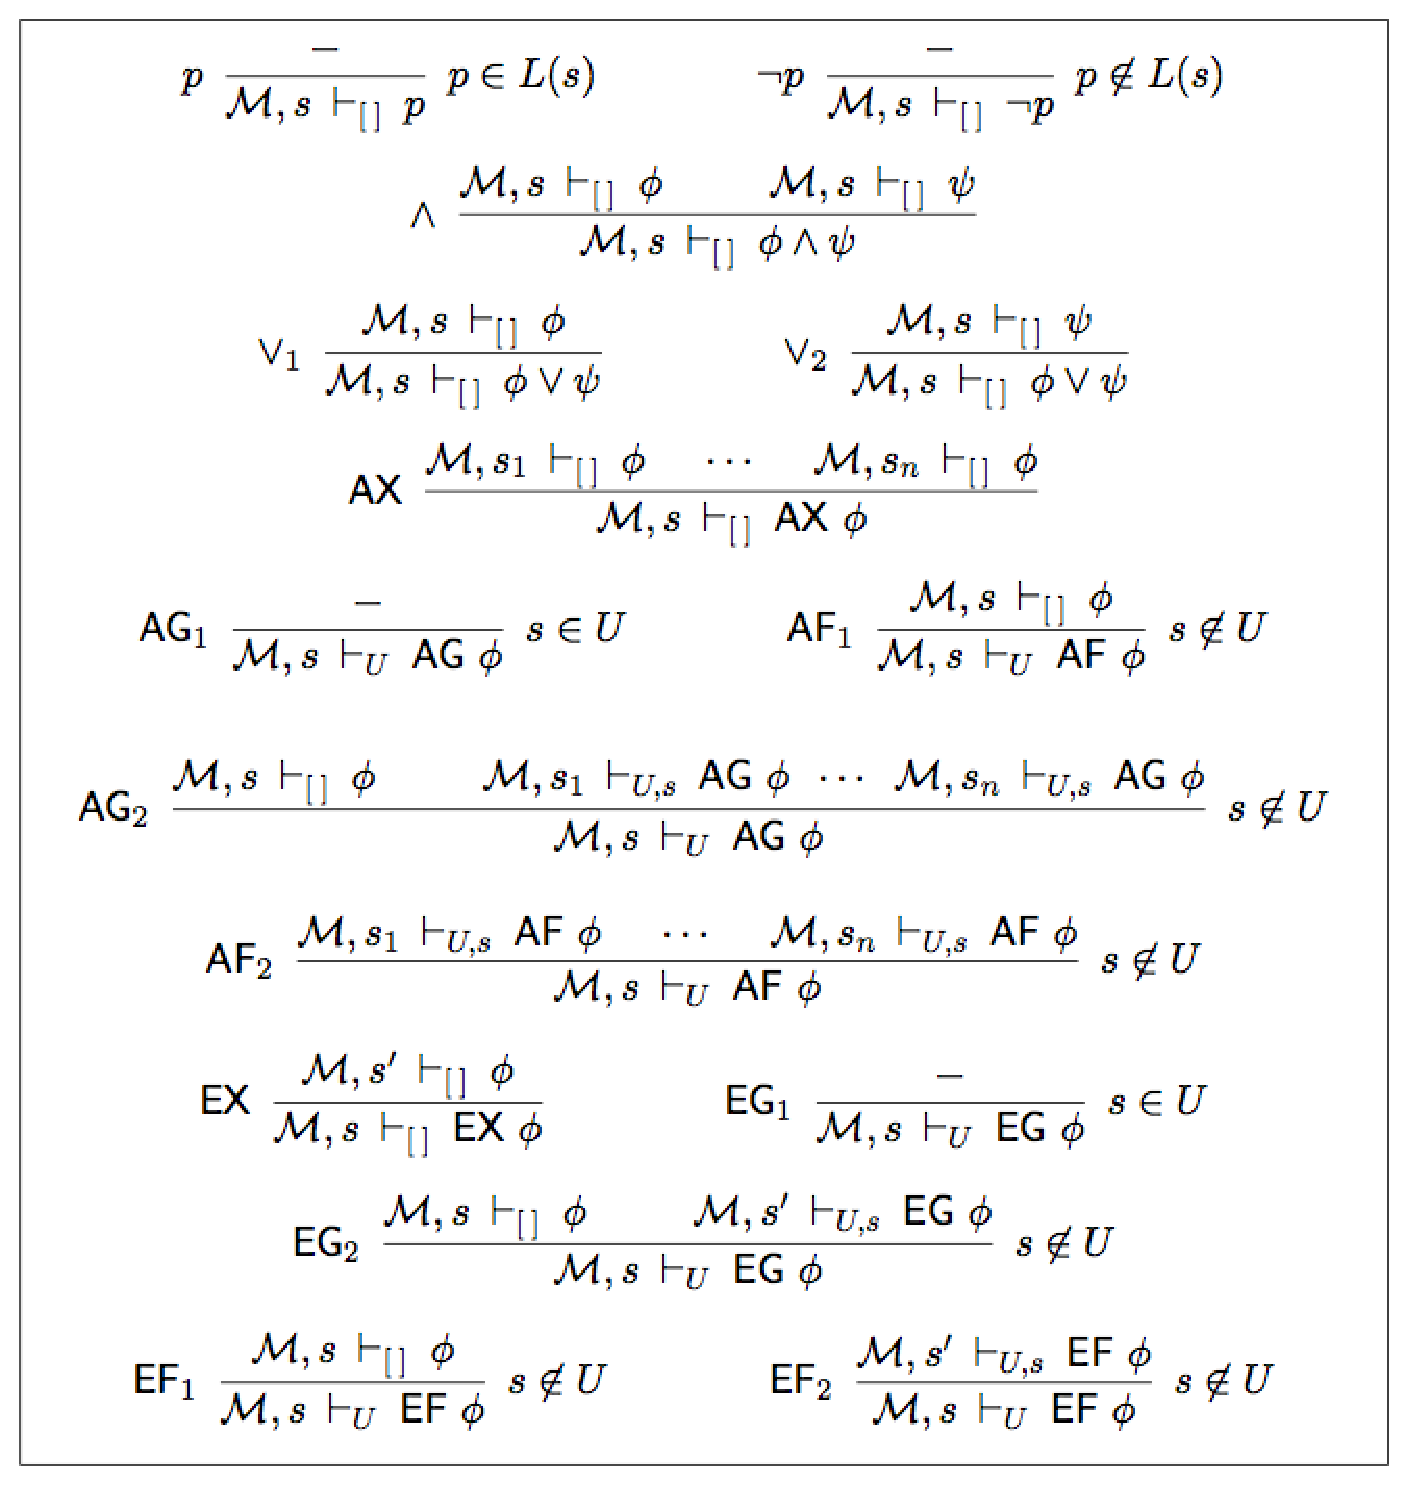
\includegraphics[width=\textwidth]{formulas.eps}
\caption{Regler för CTL}
\label{fig:ctl-regler}
\end{figure}

\subsection{Modellprovaren}\label{sub:modellprovaren}

För att kunna testa modellprovaren fanns flertalet tester att tillgå som bestod av en liststruktur för att beskriva tillståndens egenskaper och grannar, detta beskrivs tydligare under Modell.
Programmet skrevs så att en funktion “check” anropades med följande inparametrar:

\begin{center}
\begin{minipage}{0.75\textwidth}
\texttt{check(T, L, S, U, F)}

\texttt{T - Alla tillstånd och dess grannar i listform}

\texttt{L - Lista över egenskaper i varje tillstånd}

\texttt{S - Aktuellt tillstånd}

\texttt{U - Lista för besökta tillstånd}

\texttt{F - CTL formel som ska testas}

\end{minipage}
\end{center}

Check skrevs så att den med pattern matching kan matchas mot alla de regler som skulle implementeras. De matchades på följande sätt: \texttt{X}, \texttt{neg(X)}, \texttt{and(F,G)}, \texttt{or(F,G)}, \texttt{ax(X)}, \texttt{ag(X)}, \texttt{ex(X)}, \texttt{eg(X)}, \texttt{ef(X)}.

Nedan följer ett utrag ur programkoden för kontroll av \texttt{ef(X)}:

\begin{center}
\begin{minipage}{0.6\textwidth}

\begin{lstlisting}
% EF 1
check(T, L, S, U, ef(X)) :-
	not(member(S, U)),
	check(T, L, S, [], X).

% EF 2
check(T, L, S, U, ef(X)) :-
	not(member(S, U)),
	member([S, Srest], T),
	echeck(T, L, Srest, [S|U], ef(X)).
\end{lstlisting}
\end{minipage}
\end{center}

Då check stötte på \texttt{ef(X)} försökte den först med implementationen EF1 och
sedan om den evaluerades till false försökte den med EF2.

EF1 skrevs så att den alltid kontrollerar att nuvarande tillstånd \textit{S} inte finns bland tidigare besökta \textit{U} och fortsätter sedan rekursivt med resten av beviset \textit{X} och tömd lista \textit{U} för tidigare besökta tillstånd. Detta uppfyller kraven för regel EF1 som kan ses i figur 1.

EF2 skrevs så att den på samma sätt som EF1 kontrollerar att \textit{S} inte
tidigare har besökts. I nästa steg kontrollerar den vilka grannar \textit{S} har
övergångar till och skickar med dessa till funktionen echeck. Denna funktion kontrollerar att
någon av tillståndets \textit{S} grannar evalueras till sant. Till echeck skickas även en lista innehållandes tidigare besökta tillstånd där nuvarande tillståndet \textit{S} läggs till. Detta uppfyller
kraven för EF2.

De resterande reglerna från figur~\ref{fig:ctl-regler} implementerades på liknande sätt och dessa kan ses i den bifogade koden under kapitel~\ref{sub:programkod}.

\subsection{Modell}\label{sub:modell}

Den icke-triviala modellen som skapades beskiver ett trafikljus olika tillstånd. Ett trafikjus har följande sekvenser: rött \textrightarrow\ rött/gult \textrightarrow\ grönt, grönt \textrightarrow\ gult \textrightarrow\ rött, gult \textrightarrow\ släckt  \textrightarrow\ gult... och avstängt. Dessa sekvenser kan beskrivas som en modell med övergångar mellan de olika tillstånden.

I tillståndet “s0” kan trafikljuset lysa konstant rött, släckas “s5” eller gå till rött/gult “s1”. Från “s1” kan släckt tillstånd “s5”, rött “s0” och grönt “s3” nås. Då trafikljuset lyser gult i “s2” kan tillståndet rött “s0”, grönt “s3” och släckt “s5” nås. I tillståndet grönt kan det stå still, gå till gult “s2” eller släckas “s5”. Vid tekniska problem kan det blinka gult “s4”, från detta tillstånd kan endast släckt “s5” nås direkt. Då trafikljuset är släckt “s5” och ska tändas kan rött “s0” och blinkande gult “s4” nås som nästkommande tillstånd. Genom att kombinera dessa övergångar mellan tillstånden till stigar kan trafikljusets alla sekvenser skapas.

Detta beskrivs i figur~\ref{fig:ctl-states} där egenskperna i tillstånden är: \textit{r = rött, y = gult, g = grönt, o = släckt och f = blinkande}.

\begin{figure}[ht]
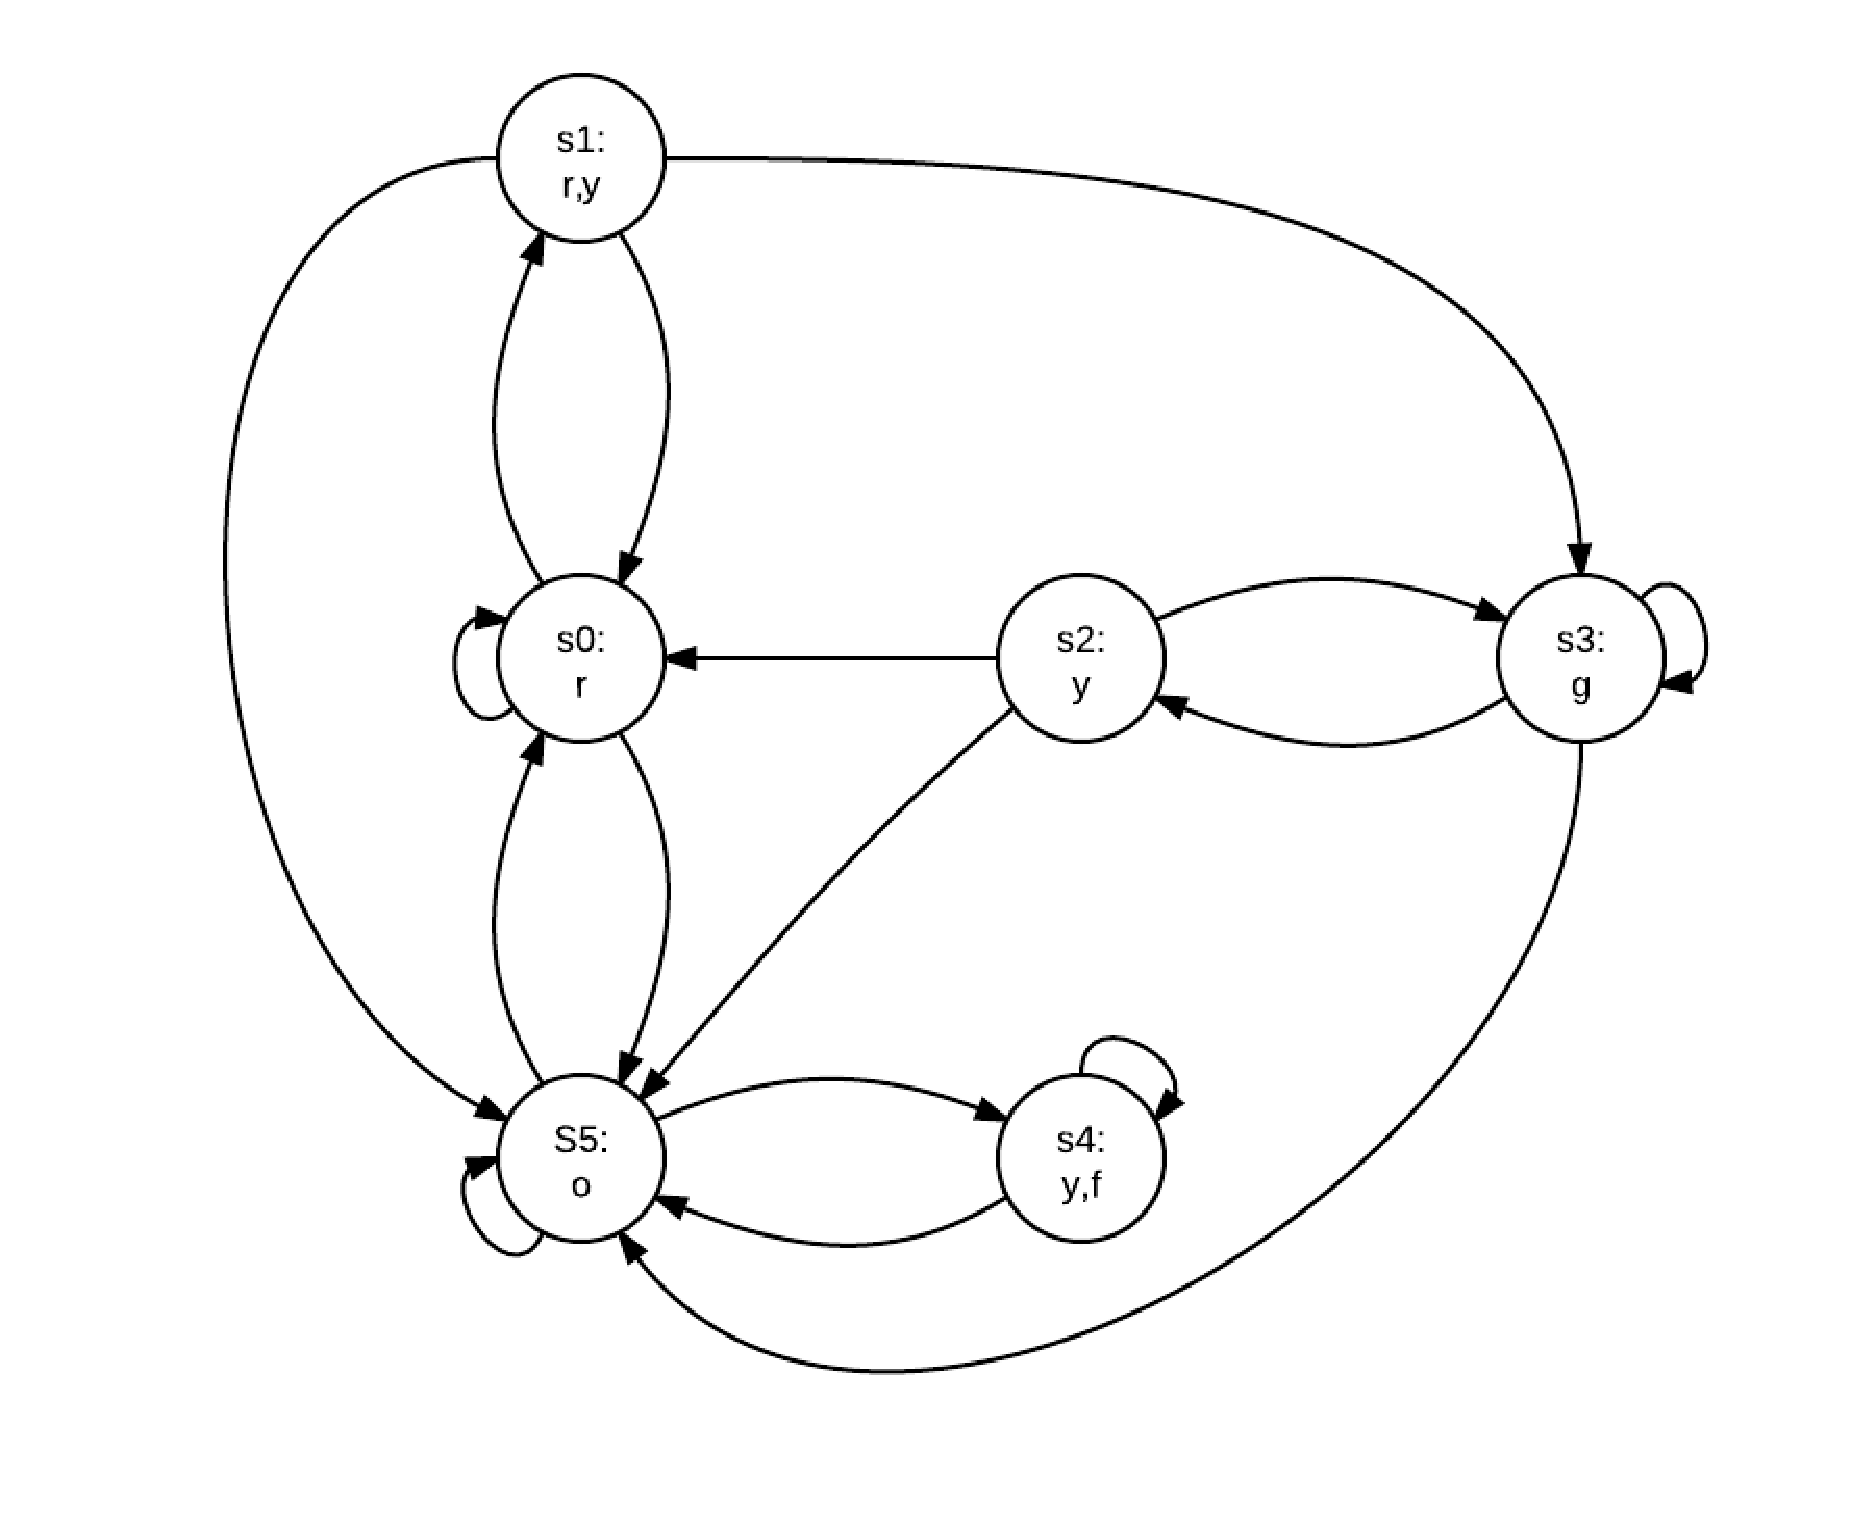
\includegraphics[width=\textwidth]{states.eps}
\caption{Tillståndsgraf}
\label{fig:ctl-states}
\end{figure}

För modellen $\mathcal{M}$ = (\textit{S},\textrightarrow,\textit{L}) är tillståndsmängden \textit{S}:

\begin{tabbing}
\textit{S} = \= \textbraceleft \textit{s0,s1,s2,s3,s4,s5}\textbraceright\\
\end{tabbing}

Transitionsrelationen \textrightarrow\ som beskriver alla grannar: 
\begin{tabbing}
\textrightarrow\ = \= \textbraceleft (\textit{s0,s0}),(\textit{s0,s1}),(\textit{s0,s5}),\\
\> (\textit{s1,s0}),(\textit{s1,s3}),(\textit{s1,s5}),\\
\> (\textit{s2,s0}),(\textit{s2,s3}),(\textit{s2,s5}),\\
\> (\textit{s3,s2}),(\textit{s3,s3}),(\textit{s3,s5}),\\
\> (\textit{s4,s4}),(\textit{s4,s5}),\\
\> (\textit{s5,s0}),(\textit{s5,s4}),(\textit{s5,s5})\textbraceright\\
\end{tabbing}

Sanningstilldelningen L som beskriver egenskaperna som finns i varje tillstånd:
\begin{tabbing}
\textit{L} = \textbraceleft\
\textit{s0}:\textbraceleft
\textit{r}\textbraceright, 
\textit{s1}:\textbraceleft 
\textit{r,y}\textbraceright, 
\textit{s2}:\textbraceleft 
\textit{y}\textbraceright, 
\textit{s3}:\textbraceleft 
\textit{g}\textbraceright, 
\textit{s4}:\textbraceleft 
\textit{y,f}\textbraceright, 
\textit{s5}:\textbraceleft 
\textit{o}\textbraceright\ \textbraceright
\end{tabbing}

Denna modell översattes till lämplig listsruktur som de övriga testerna för att fungera med den i prolog implementerade beviskontrolleraren.
\begin{tabbing}
Transitionsrelationen (\textit{T}):
[\=[\textit{s0}, [\textit{s0, s1 ,s5}]],\\
\>[\textit{s1}, [\textit{s0, s3, s5}]],\\
\>[\textit{s2}, [\textit{s0, s1, s3, s5}]],\\
\>[\textit{s3}, [\textit{s3, s2, s5}]],\\
\>[\textit{s4}, [\textit{s4, s5}]],\\
\>[\textit{s5}, [\textit{s5, s0, s4, s5}]]].\\
\end{tabbing}

\begin{tabbing}
Sanningstilldelningen (\textit{L}):
[\=[\textit{s0}, [\textit{r}]],\\
\>[\textit{s1}, [\textit{r,y}]],\\
\>[\textit{s2}, [\textit{y}]],\\
\>[\textit{s3}, [\textit{g}]],\\
\>[\textit{s4}, [\textit{y,f}]],\\
\>[\textit{s5}, [\textit{o}]]].\\
\end{tabbing}

För denna modell skapades två stycken CTL-formler, en som stämmer och en som inte stämmer.
Formeln \texttt{ef(ag(ex(o)))} är korrekt och innebär: "det finns en stig där det så småningom alltid finns en stig där det i något nästa tillstånd gäller att trafikljuset är avstängt", dvs. Var vi än är kan trafikljuset på något sätt stängas av. Den formel som är felaktig \texttt{and(r,ax(g))} innebär: det finns ett tillstånd där bara rött gäller och i nästa tillstånd gäller bara grönt. Detta betyder att man skulle kunna gå direkt från rött till grönt vilket inte stämmer då den enda vägen dit är via tillståndet då både röd och gul signal ges.